\documentclass{article}
\usepackage{calc}
\usepackage{graphicxsp}

%
% Since you are using distiller, you have Acrobat as well.
% Try using the PDF Optimizer to further reduce the size
% of the file. If you have Acrobat Pro 8.0, you can do
% a Save As, by selecting Adobe PDF Files, Optimized
% from the Save as type list. This is the same as using
% the PDF Optimizer.
%

\newcommand{\cs}[1]{\texttt{\char`\\#1}}

\special{!userdict begin
    /Draw_Ellipse {
        /m matrix currentmatrix def
        4 2 roll translate scale
        0 0 1 0 360 arc
        closepath
        m setmatrix
    } def end
}

\embedEPS[hiresbb,transparencyGroup]{AdobeDon}{graphics/AdobeDon}   % 284 KB
\embedEPS[hiresbb,transparencyGroup]{Airplane}{graphics/000_0151}   % 550 KB
\embedEPS[hiresbb]{AdobeDon_full}{graphics/AdobeDon_full}           % 370 KB
\embedEPS[transparencyGroup]{ex}{graphics/example}                  % 7.7 KB


\parindent0pt
\setlength{\fboxsep}{0pt}

\thispagestyle{empty}

\begin{document}

\begin{center}
The GraphicxSP Package\\
D. P. Story
\end{center}

The package, tentatively named \textsf{graphicxsp} and which is still under development,
attempts to use the PostScript operators \textbf{BP}, \textbf{EP} and \textbf{SP} to embed
graphics in the document once, then use and re-use them by emitting the \textbf{SP} operator.
Though this document was created using \textsf{AeB Pro}, the package only requires
the \textsf{graphicx} and \textsf{eso-pic} packages.

\medskip
We begin by embedding out graphics in the preamble of the document using the
\cs{embedEPS} command. The command takes one optional argument and two required. We can
not only use these graphics over again, the package does support transparency as well, as
this file also demonstrates.
\begin{small}
\begin{verbatim}
\embedEPS[hiresbb,transparencyGroup]{AdobeDon}{AdobeDon}    % 284 KB
\embedEPS[hiresbb,transparencyGroup]{Airplane}{000_0151}    % 550 KB
\embedEPS[hiresbb]{AdobeDon_full}{AdobeDon_full}            % 370 KB
\embedEPS[transparencyGroup]{ex}{example}                   % 7.7 KB
\end{verbatim}
\end{small}

% Normal,Multiply, Screen, Screen, Darken, Lighten, ColorDodge, ColorBurn, HardLight,
% SoftLight, Difference, Exclusion


The package attempts to blend in with the \textsf{graphicx} package, and uses
the \cs{includegraphics} command, with a few extra optional key-value
pairs.
\begin{small}%
\begin{verbatim}
\insertEPS[width=1.5in]{AdobeDon}
\includegraphics*[name=AdobeDon,angle=45,
    width=1.5in,bb=30 50 150 100]{AdobeDon}
\end{verbatim}
\end{small}%



\begin{center}
\insertEPS[width=1.5in]{AdobeDon}
\includegraphics*[name=AdobeDon,width=1.5in,angle=45,bb=30 50 150 100]{AdobeDon}
\end{center}
The second command is in the form of \cs{includegraphics}, the first
one, \cs{embedEPS}, is a shortened version. After embedding, the file name is no longer used,
only the symbolic name.

Let's have some fun with two of these images.

\vspace*{.5in}

\begin{center}%\previewtrue
\begin{minipage}{.5\linewidth}
\begin{center}
\makebox[0pt][l]{\rotatebox[origin=lb]{180}{\smash{\insertEPS[width=1in]{Airplane}}}}%
\makebox[0pt][l]{\rotatebox[origin=lb]{150}{\smash{\insertEPS[width=1in]{Airplane}}}}%
\makebox[0pt][l]{\rotatebox[origin=lb]{135}{\smash{\insertEPS[width=1in]{Airplane}}}}%
\makebox[0pt][l]{\rotatebox[origin=lb]{120}{\smash{\insertEPS[width=1in]{Airplane}}}}%
\makebox[0pt][l]{\rotatebox[origin=lb]{90}{\smash{\insertEPS[width=1in]{Airplane}}}}%
\makebox[0pt][l]{\rotatebox[origin=lb]{60}{\smash{\insertEPS[width=1in]{Airplane}}}}%
\makebox[0pt][l]{\rotatebox[origin=lb]{45}{\smash{\insertEPS[width=1in]{Airplane}}}}%
\makebox[0pt][l]{\rotatebox[origin=lb]{30}{\smash{\insertEPS[width=1in]{Airplane}}}}%
\makebox[0pt][l]{\insertEPS[width=1in]{Airplane}}%
\end{center}
\end{minipage}\hfill%
\begin{minipage}{.5\linewidth}
\begin{center}
\makebox[0pt][l]{\rotatebox[origin=lb]{180}{\smash{\insertEPS[width=1in]{AdobeDon}}}}%
\makebox[0pt][l]{\rotatebox[origin=lb]{150}{\smash{\insertEPS[width=1in]{AdobeDon}}}}%
\makebox[0pt][l]{\rotatebox[origin=lb]{135}{\smash{\insertEPS[width=1in]{AdobeDon}}}}%
\makebox[0pt][l]{\rotatebox[origin=lb]{120}{\smash{\insertEPS[width=1in]{AdobeDon}}}}%
\makebox[0pt][l]{\rotatebox[origin=lb]{90}{\smash{\insertEPS[width=1in]{AdobeDon}}}}%
\makebox[0pt][l]{\rotatebox[origin=lb]{60}{\smash{\insertEPS[width=1in]{AdobeDon}}}}%
\makebox[0pt][l]{\rotatebox[origin=lb]{45}{\smash{\insertEPS[width=1in]{AdobeDon}}}}%
\makebox[0pt][l]{\rotatebox[origin=lb]{30}{\smash{\insertEPS[width=1in]{AdobeDon}}}}%
\makebox[0pt][l]{\insertEPS[width=1in]{AdobeDon}}%
\end{center}
\end{minipage}
\end{center}

\vspace{1in}

Wow! That would normally take up gobs of file space. This file is about 180 KB.

\def\mypreSP#1{%
    newpath
    \widthOf{#1} 2 div \heightOf{#1} 2 div
    \widthOf{#1} 2 div \heightOf{#1} 2 div
    Draw_Ellipse
    clip
    newpath
}
\def\mypostSP#1{%
    gsave
    [ /ca .6 /CA .3 /BM/Screen /SetTransparency pdfmark
    \widthOf{#1} 2 div \heightOf{#1} 2 div
    \widthOf{#1} 2 div \heightOf{#1} 2 div
    Draw_Ellipse
    0.4 0.7 1 setrgbcolor
    fill
    grestore
    gsave
    [ /CA .5 /BM /Normal /SetTransparency pdfmark
    \widthOf{#1} 2 div \heightOf{#1} 2 div
    \widthOf{#1} 2 div \heightOf{#1} 2 div
    Draw_Ellipse
    40 setlinewidth
    0.4 0.7 1 setrgbcolor
    stroke
    grestore
}

\medskip
Let's try some clipping with some transparency settings.

\medskip
\begin{minipage}{1.6in}
\begin{center}
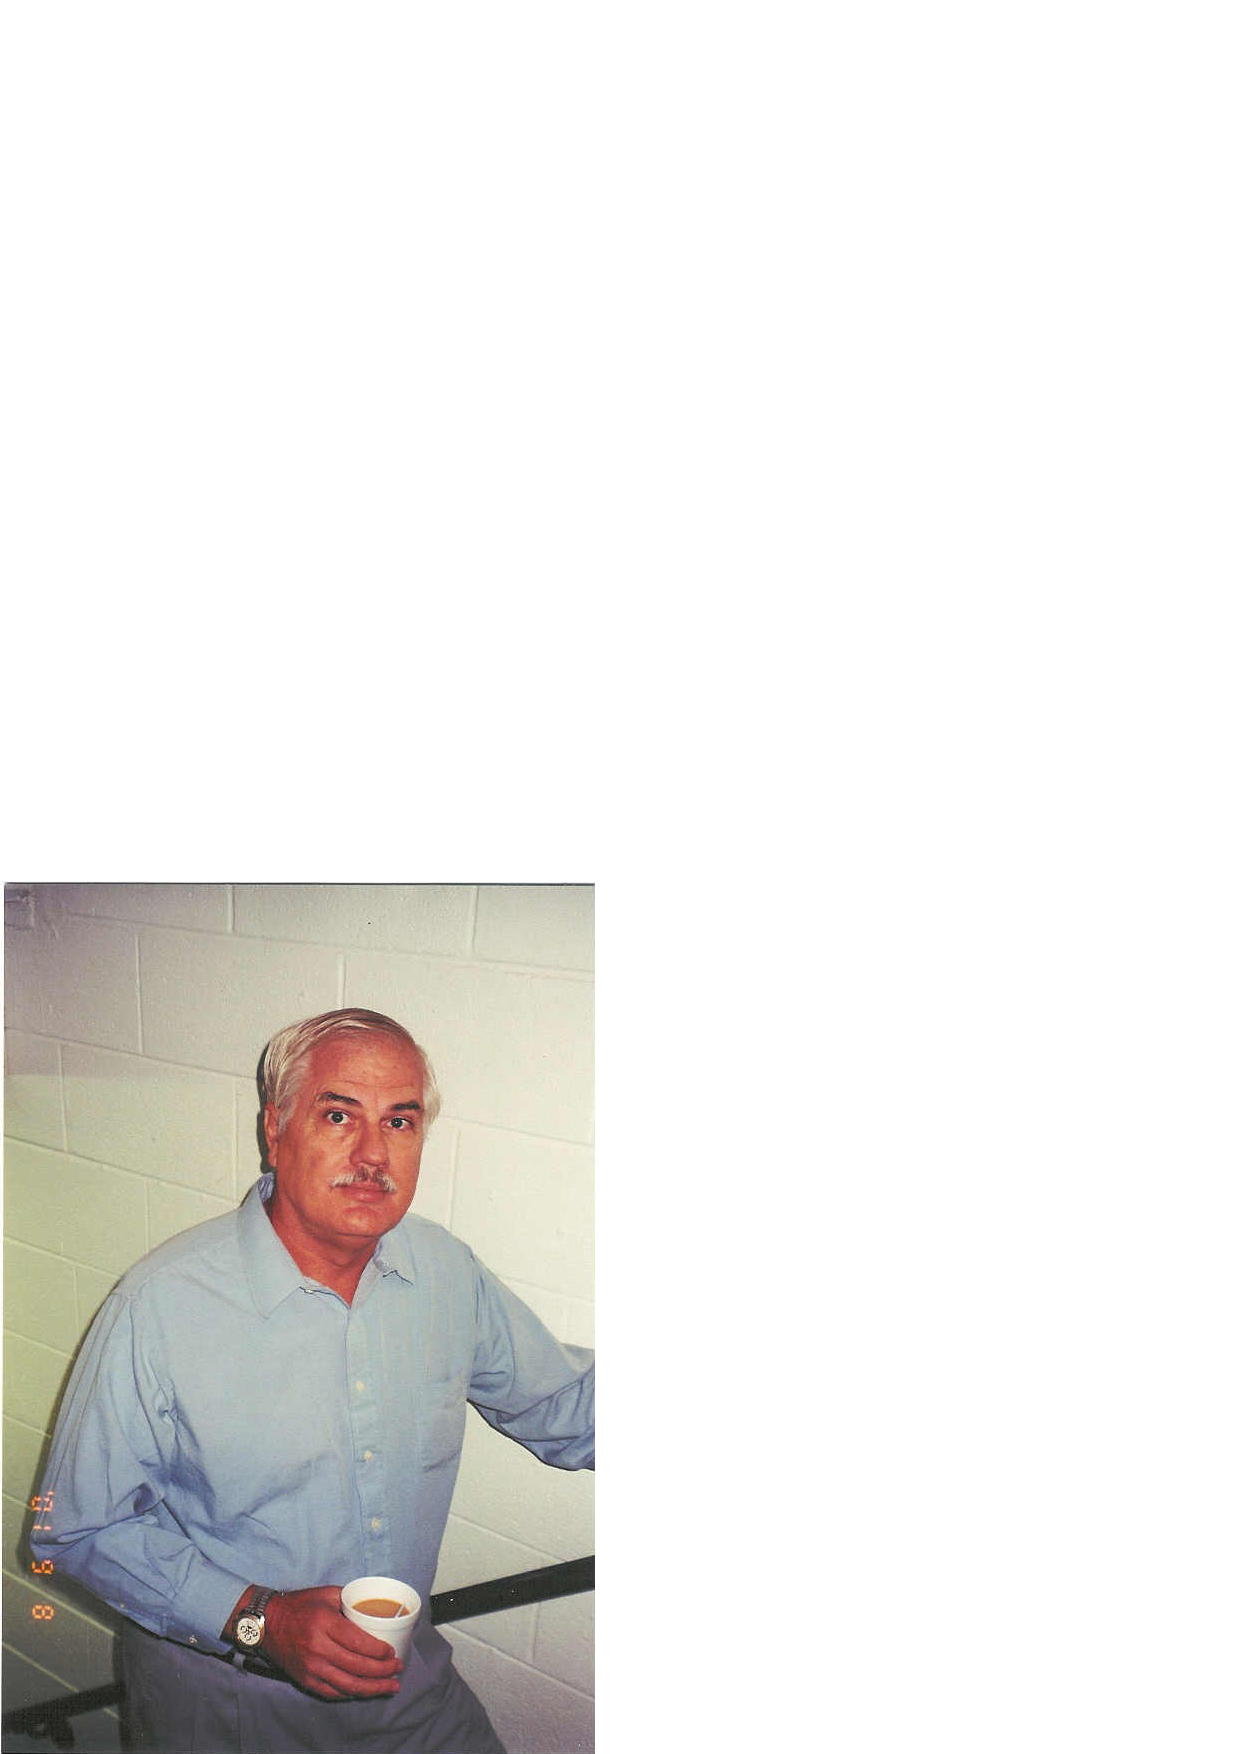
\includegraphics[name=AdobeDon_full,width=1.5in,
    presp={\mypreSP{AdobeDon_full}},
    postsp={\mypostSP{AdobeDon_full}}]{AdobeDon_full}
\end{center}
\end{minipage}\hfill
\begin{minipage}{\linewidth-1.6in}\scriptsize
\begin{verbatim}
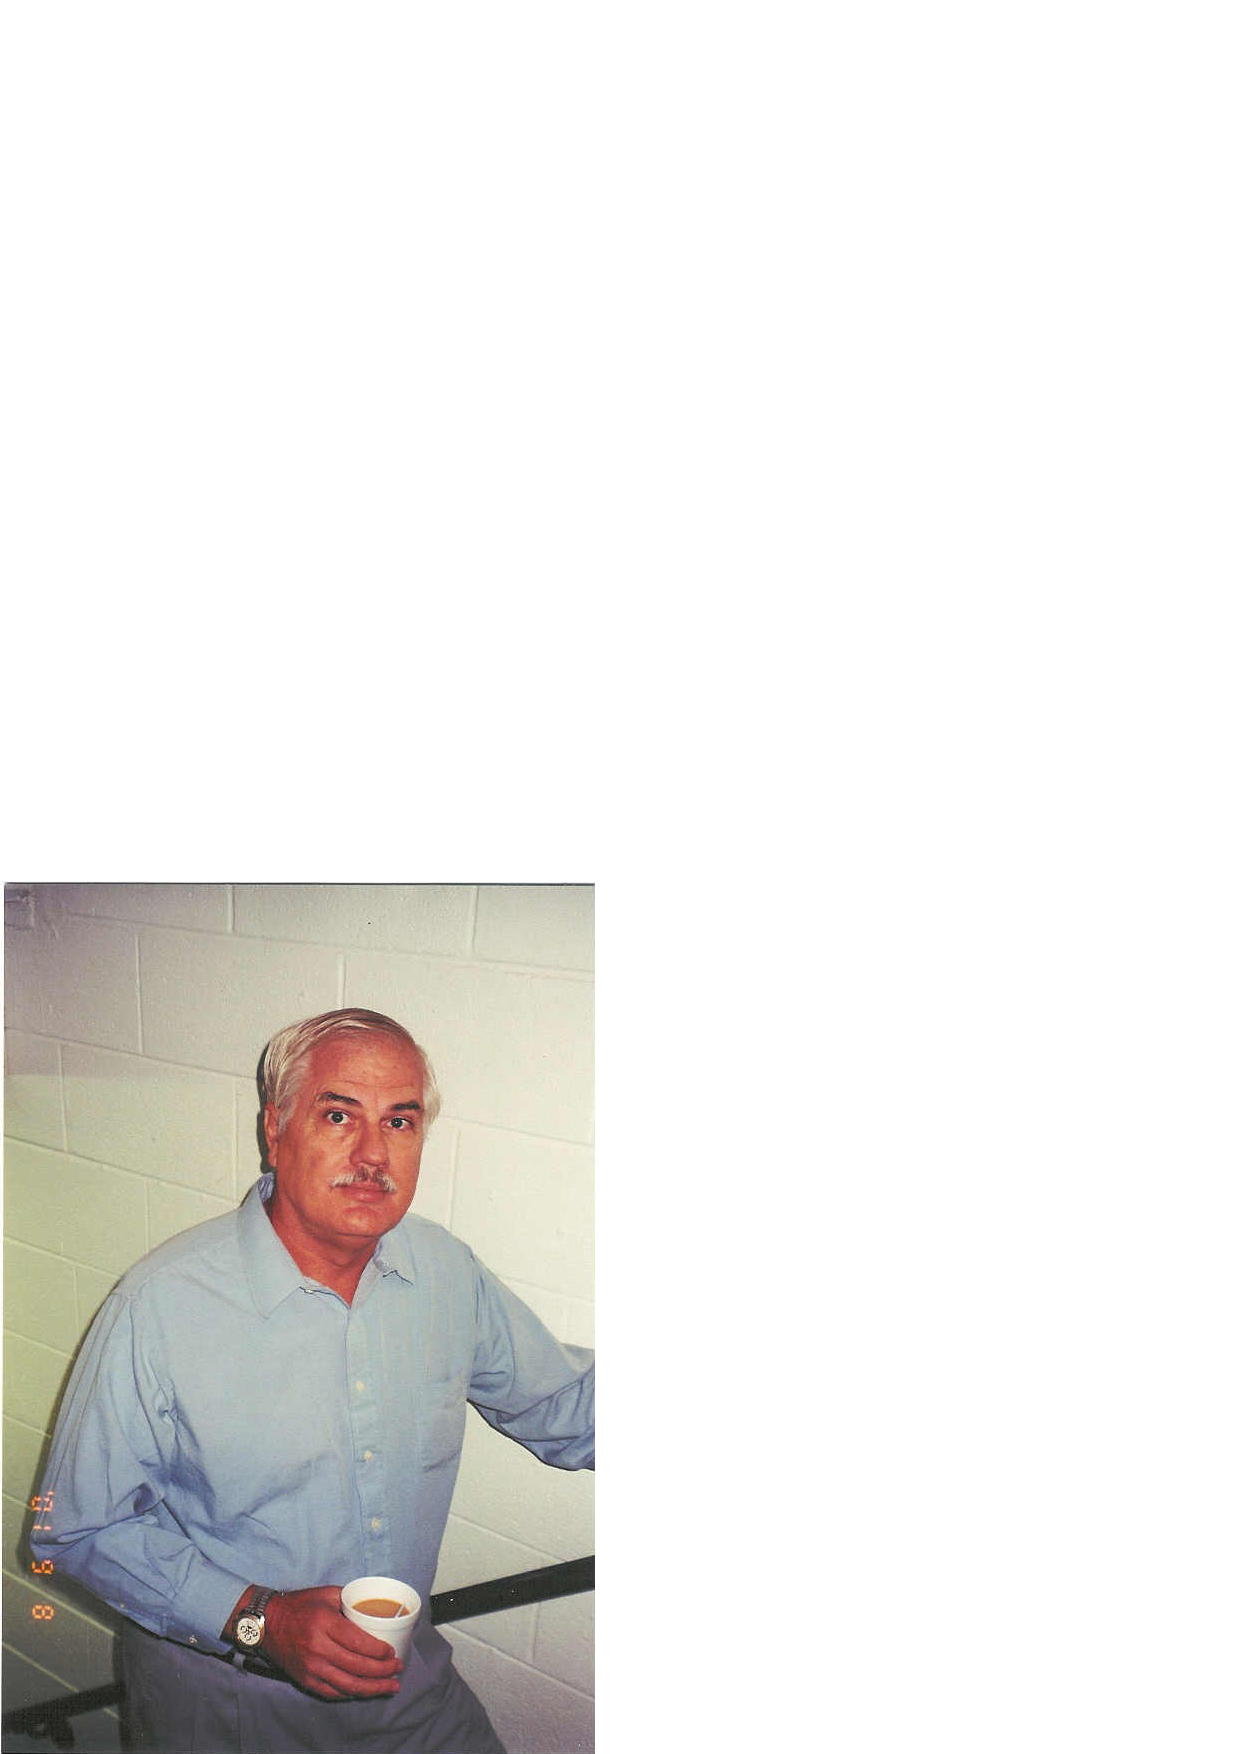
\includegraphics[name=AdobeDon_full,width=1.5in,
    presp={\mypreSP{AdobeDon_full}},
    postsp={\mypostSP{AdobeDon_full}}]{AdobeDon_full}
\end{verbatim}
{\normalsize where}
\begin{verbatim}
\def\mypreSP#1{%
    newpath
    \widthOf{#1} 2 div \heightOf{#1} 2 div
    \widthOf{#1} 2 div \heightOf{#1} 2 div
    Draw_Ellipse clip newpath
}
\def\mypostSP#1{%
    gsave
    [ /ca .6 /CA .3 /BM/Screen /SetTransparency pdfmark
    \widthOf{#1} 2 div \heightOf{#1} 2 div
    \widthOf{#1} 2 div \heightOf{#1} 2 div
    Draw_Ellipse 0.4 0.7 1 setrgbcolor fill
    grestore gsave
    [ /CA .5 /BM /Normal /SetTransparency pdfmark
    \widthOf{#1} 2 div \heightOf{#1} 2 div
    \widthOf{#1} 2 div \heightOf{#1} 2 div
    Draw_Ellipse 40 setlinewidth
    0.4 0.7 1 setrgbcolor stroke
    grestore
}
\end{verbatim}
\end{minipage}
Demonstrating some transparent special effects. Swave!

\begin{center}
\texttt{AdobeDon} and \texttt{AdobeDon} with 50\% opacity\\[1ex]
\insertEPS[width=1.5in]{AdobeDon} \insertEPS[width=1.5in,transparency={/ca .5 /BM/Normal}]{AdobeDon}
\end{center}


\begin{center}\previewtrue
\textsf{\textbf{MathLab Graphics}}\\[1ex]
\insertEPS[width=1in]{ex}  \insertEPS[width=1in,clip]{ex} \insertEPS[width=1in,transparency={/ca .3}]{ex}\\
\end{center}
The bounding box for this graphic is
\texttt{[\llxOf{ex}\space\llyOf{ex}\space\urxOf{ex}\space\uryOf{ex}]}.
The figure in the middle has been clipped using its bounding box (the \texttt{clip} option
of \cs{insertEPS} and \cs{includegraphics)}, the
one on the right has 30\% opacity and has not been clipped.
\end{document}

\margins{.25in}{.25in}{24pt}{.25in} % left,right,top, bottom
\screensize{5.4in*\real{0.75}}{5in} % height, width
